\documentclass[11pt, a4paper]{article}
\usepackage{graphicx}
\usepackage{amsmath}
\usepackage[margin=0.6in]{geometry}
\usepackage{listings}
\usepackage{float}

\title{EE2703: Assignment 3} % Title
\author{Akilesh Kannan (EE18B122)} % Author name
\date{February 5, 2020} % Date for the report

\begin{document}
    \maketitle % Insert the title, author and date

    \section{Aim}
        In this assignment we aim to :
        \begin{itemize}
            \item Observe the error in fitting the \textit{Least Error Fit} function to a given set of data.
            \item Find the relation between the error observed and the noise in the data.
        \end{itemize}

    \section{Procedure}
        The function to be fitted is:
        \begin{equation*}
            f(t) = 1.05J_2(t)-0.105t
        \end{equation*}
        where $J_2(t)$ is the \textit{Bessel Function of the first kind of Order 2}. The true data used for fitting is obtained using this equation.

        \subsection{Creating noisy data}
            To create the noisy data, we add random noise to $f(t)$. This random noise, denoted by $n(t)$, is given by the standard normal probability distribution:
            \begin{equation}
                P(n(t)|\sigma)=\frac{1}{\sqrt{2\pi\sigma^2}}e^{-\frac{n(t)^2}{2\sigma^2}} \label{eq1}
            \end{equation}
            The resulting noisy data will be of the form:
            \begin{equation}
                f(t) = 1.05J_2(t)-0.105t+n_{\sigma_i}(t)
            \end{equation}
            where, $n_{\sigma_i}(t)$ is the noisy data function with $\sigma = \sigma_{i}$ in \eqref{eq1}. Thus for 9 different values of sigma (in a log scale from 0.001 to 0.1), the noisy data is created and stored in the \texttt{\textbf{fitting.dat}} file.

        \subsection{Analyzing the noisy data}
            The data is read and plotted using PyPlot. The output result looks as follows:
            \begin{figure}[H]
                \centering
                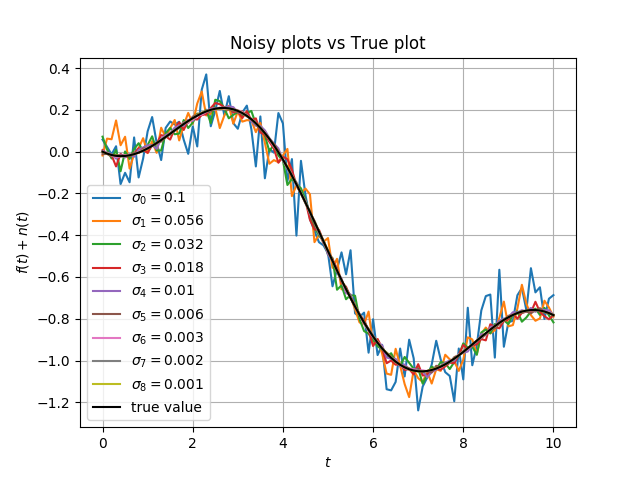
\includegraphics[scale=0.5]{Fig 0.png}
                \caption{Noisy Data with True Data}
                \label{fig:noisyAndTrue}
            \end{figure}

            As we can see, the ``noisiness'' of the data increases with increasing value of $\sigma$. Another view of how the noise affects the data can be seen below:
            \begin{figure}[H]
                \centering
                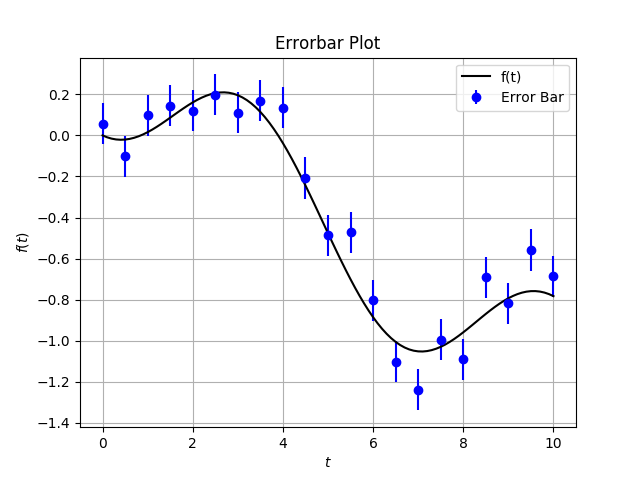
\includegraphics[scale=0.5]{Fig 1.png}
                \caption{Noisy Data with Errorbar}
                \label{fig:noiseError}
            \end{figure}

            The blue lines (\textit{error bar}) indicate the standard deviation of the noisy data from the original data, at that value of $t$. It is plotted at every $5^\text{th}$ point to make the plot readable.

        \subsection{Finding the best approximation for the noisy data}
            From the data, we can conclude that the data can be fitted into a function of the form:
            \begin{equation}
                g(t, A, B) = AJ_2(t)+Bt
            \end{equation}
            where $A$ and $B$ are constants that we need to find.\\

            To find the coefficients $A$ and $B$, we first try to find the mean square error between the function and the data for a range of values of \textit{A} and \textit{B}, which is given by:
            \begin{equation}
                \epsilon_{ij} = \frac{1}{101}\sum_{k=0}^{101}(f(t_k) - g(t_k, A_i, B_j))^2
            \end{equation}
            where $\epsilon_{ij}$ is the error for $(A_i,B_j)$. The contour plot of the error is shown below:
            \begin{figure}[H]
                \centering
                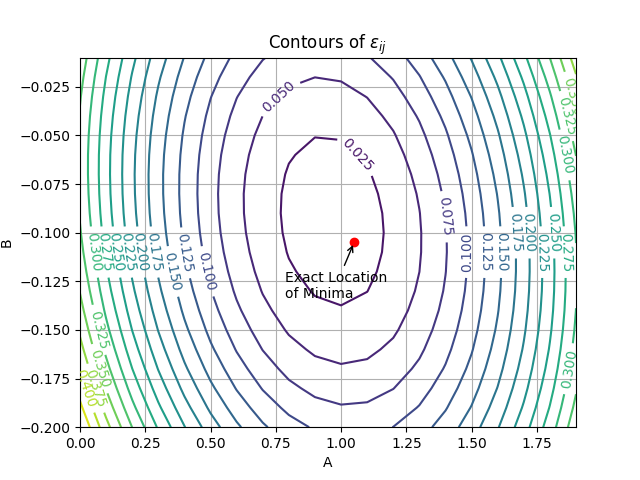
\includegraphics[scale=0.5]{Fig 2.png}  % Mention the image name within the curly braces. Image should be in the same folder as the tex file.
                \caption{Contour Plot of $\epsilon_{ij}$}
                \label{fig:contourPlot}
            \end{figure}

            We can see the location of the minima to be approximately near the orignal function coefficients.\\

            Using the \texttt{lstsq} function in \texttt{scipy} package, we solve for:
            \begin{equation}
            M.p = D \label{eq5}
            \end{equation}
            where
            \begin{equation}
            M=\left[\begin{matrix}
            J_2(t_1)&t_1\\
            ...&...\\
            J_2(t_m)&t_m
            \end{matrix}\right]\text{, }p=\left[\begin{matrix}
            A_{fit}\\B_{fit}
            \end{matrix}\right]\ \text{and }D=\left[\begin{matrix}f(t_1)\\...\\f(t_m)\end{matrix}\right]
            \end{equation}\\

            Thus, we solve for $p$ and then find the mean square error of the values of $A_{fit}$ and $B_{fit}$ found using \texttt{lstsq} and the original values $(1.05,\ -0.105)$.

        \subsection{Finding out the variation of $\epsilon$ with $\sigma_n$}
            We solve \eqref{eq5} for different values of $\sigma_n$, by changing matrix D to different columns of \texttt{\textbf{fitting.dat}}. We find that the variation of the mean squared error of values $A_{fit}$ and $B_{fit}$ is as follows:
            \begin{figure}[H]
                \centering
                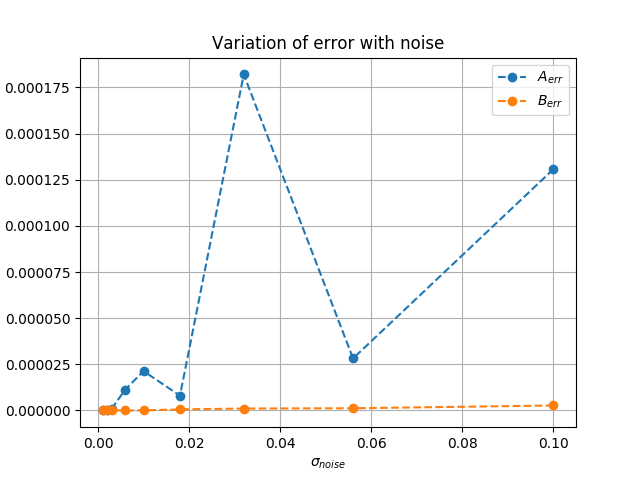
\includegraphics[scale=0.5]{Fig 3.png}  % Mention the image name within the curly braces. Image should be in the same folder as the tex file.
                \caption{Mean Squared Error vs Standard Deviation}
                \label{fig:errorSTD}
            \end{figure}

            This plot does not give that much useful information between $\sigma_n$ and $\epsilon$, but when we do the \texttt{loglog} plot as below:
            \begin{figure}[H]
                \centering
                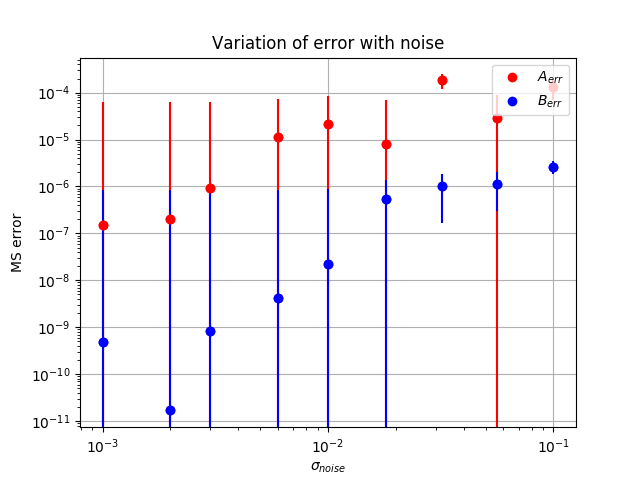
\includegraphics[scale=0.5]{Fig 4.png}  % Mention the image name within the curly braces. Image should be in the same folder as the tex file.
                \caption{Error vs Standard Deviation \texttt{loglog} Plot}
                \label{fig:errorSTDloglog}
            \end{figure}

            We can see an approximately linear relation between $\sigma_n$ and $\epsilon$. This is the required result.

    \section{Conclusion}
        From the above procedure, we were able to determine that \textbf{the logarithm of the standard deviation of the noise} \textit{\textbf{linearly affects}} \textbf{the logarithm of the error} in the calcuation of the least error fit for a given data.
\end{document}
